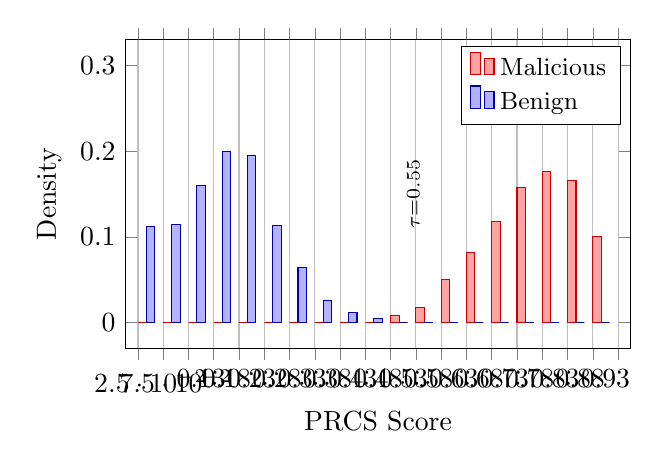
\begin{tikzpicture}
\begin{axis}[
  ybar interval,
  width=8cm, height=5.5cm,
  xlabel={PRCS Score},
  ylabel={Density},
  xmin=0, xmax=1,
  legend style={at={(0.98,0.98)}, anchor=north east, font=\small},
  legend cell align={left},
]
\addplot[fill=red!60, fill opacity=0.6, draw=red!80!black]
  coordinates {(0.0250,0.000000) (0.0750,0.000000) (0.1250,0.000000) (0.1750,0.000000) (0.2250,0.000000) (0.2750,0.000000) (0.3250,0.000000) (0.3750,0.000000) (0.4250,0.000000) (0.4750,0.000000) (0.5250,0.008000) (0.5750,0.018000) (0.6250,0.050000) (0.6750,0.082000) (0.7250,0.118000) (0.7750,0.158000) (0.8250,0.176000) (0.8750,0.166000) (0.9250,0.100000) (0.9750,0.124000)};
\addlegendentry{Malicious}
\addplot[fill=blue!50, fill opacity=0.6, draw=blue!70!black]
  coordinates {(0.0250,0.111932) (0.0750,0.114044) (0.1250,0.159979) (0.1750,0.200106) (0.2250,0.195354) (0.2750,0.112988) (0.3250,0.063886) (0.3750,0.025343) (0.4250,0.011616) (0.4750,0.004752) (0.5250,0.000000) (0.5750,0.000000) (0.6250,0.000000) (0.6750,0.000000) (0.7250,0.000000) (0.7750,0.000000) (0.8250,0.000000) (0.8750,0.000000) (0.9250,0.000000) (0.9750,0.000000)};
\addlegendentry{Benign}
% Decision threshold line
\addplot[black, dashed, very thick]
  coordinates {(0.55,0)(0.55,0.30)};
\node[font=\scriptsize, rotate=90] at (axis cs:0.57,0.15)
  {$\tau{=}0.55$};
\end{axis}
\end{tikzpicture}